% =====================================================================
%  MLE-AI-201 Machine Learning -- Final Project
% =====================================================================
\documentclass[10pt,twocolumn,a4paper]{article}

\usepackage[a4paper,top=0.75in,bottom=1.0in,left=0.68in,right=0.68in,columnsep=0.25in]{geometry}
\usepackage{mathptmx}
\usepackage[T1]{fontenc}
\usepackage[utf8]{inputenc}
\usepackage{graphicx}
\usepackage{amsmath,amssymb}
\usepackage{booktabs}
\usepackage{array}
\usepackage{titlesec}
\usepackage{caption}
\usepackage{cite}
\usepackage[hidelinks]{hyperref}
\usepackage{url}
\usepackage{placeins}
\graphicspath{{figures/}{report/figures/}}

\renewcommand{\thesection}{\Roman{section}}
\renewcommand{\thesubsection}{\Alph{subsection}}
\titleformat{\section}[block]{\centering\normalsize\scshape}{\thesection.}{0.5em}{}
\titleformat{\subsection}[block]{\normalsize\itshape}{\thesubsection.}{0.5em}{}
\titlespacing*{\section}{0pt}{1.4ex plus 1ex minus .2ex}{1ex}
\titlespacing*{\subsection}{0pt}{1.0ex plus 1ex minus .2ex}{0.6ex}
\newcommand{\abstractkw}[1]{\noindent\textbf{\textit{#1}}}
\captionsetup{font=small,labelsep=period}
\setlength{\parindent}{1em}

\begin{document}

\twocolumn[
  \begin{@twocolumnfalse}
  \begin{center}
    {\LARGE\bfseries Real-Estate Price Prediction and Price-Tier Classification\par}
    \vspace{1.2em}
    {\large Gunel Garayzade\quad Jale Afandiyeva\quad Kheyransa Grochuyeva\quad Nazrin Burziyeva\par}
    \vspace{0.5em}
    {\itshape MLE-AI-201 Machine Learning, AI Academy --- Cohort II\par}
    \vspace{0.3em}
    {\small 18.10.2026\par}
    \vspace{1.4em}
  \end{center}
  \begin{quote}
    \small
    \abstractkw{Abstract---}
    This project studies two related tasks on bina.az real-estate listings:
    predicting the advertised price and classifying a listing as standard or
    premium. We implemented a decision tree and a Pegasos support-vector
    machine from scratch using NumPy, and compared them with matched
    scikit-learn baselines. The final pipeline removes duplicate listings,
    parses numeric and categorical fields, removes target-derived columns,
    and uses deterministic train, validation, and test partitions. On the
    held-out test set, the custom raw-price tree achieved an RMSE of
    71,741 AZN, an MAE of 48,559 AZN, and an $R^2$ of 0.660. The custom
    tree classifier achieved an F1 score of 0.873 and ROC-AUC of 0.943.
    The tree and its scikit-learn counterpart produced almost identical
    results, supporting the correctness of the implementation. The
    regression errors remain substantial for high-priced listings, so the
    model is useful for approximate estimation rather than professional
    valuation. Log-price models were also evaluated as a sensitivity
    analysis, but did not improve the main test-set results.
    The repository is available at
    \href{https://github.com/nazrinburz/mle-ai-final-project}{\texttt{github.com/nazrinburz/mle-ai-final-project}}.

    \vspace{0.6em}
    \abstractkw{Index Terms---}decision tree, support-vector machine,
    Pegasos, regression, classification, real-estate price prediction.
  \end{quote}
  \vspace{1.0em}
  \end{@twocolumnfalse}
]

\section{Introduction}
Online property listings contain useful information about location, size,
rooms, building structure, and condition, but exact price prediction is
difficult because prices are heterogeneous and some important quality
factors are not recorded. This project uses the bina.az dataset to build
two models from scratch. Task A predicts the listing price in AZN, while
Task B predicts whether the listing is above the training-set median price.

Our contributions are: (i) a NumPy decision tree supporting classification
and regression criteria; (ii) a NumPy Pegasos SVM with a Random Fourier
Feature extension; (iii) a reproducible preprocessing and evaluation
pipeline; and (iv) matched scikit-learn comparisons and error analysis.

\section{Related Work / Background}
Decision trees recursively split the feature space. For classification, a
split can reduce Gini impurity or entropy; for regression, it reduces the
within-node mean squared error. A leaf predicts the majority class or the
mean target of the observations reaching it. Depth and minimum leaf size
control the bias--variance trade-off.

The SVM separates classes using a maximum-margin decision boundary while
penalising violations of the margin. We optimise the regularised hinge-loss
objective with the Pegasos stochastic sub-gradient method
\cite{pegasos,cortes1995}. Random Fourier Features provide a finite-dimensional
approximation of an RBF feature map, allowing the same linear Pegasos
solver to model nonlinear boundaries. Random forests combine bootstrapped
trees and average their predictions to reduce variance
\cite{breiman2001}; Ridge regression provides a regularised linear baseline
\cite{hoerl1970}. These methods give useful comparisons to the two required
from-scratch models.

\section{Data and Preprocessing}
The source is a joined export of bina.az listings from the binaaz-sale
project dataset~\cite{binaaz}. The final run started
with 100,775 rows, removed 36,321 repeated listing rows, and retained
59,697 rows for evaluation after the shared cleaning pipeline. Prices and
areas were parsed from text, positive-price rows were retained, exact
duplicates were removed, and price outliers were filtered with the
1.5-IQR rule. Missing numeric values were imputed, while categorical
variables received explicit encoded categories. The design matrix contains
167 numeric or one-hot encoded features, including latitude, longitude,
area, rooms, land area, floor, total floors, renovation, city, location,
and property category.

The preprocessing also preserves information about missing floors. For
apartments, missing floor values are filled using the median for the
corresponding apartment category; for non-apartment listings, zero is used
as a not-applicable value and a missingness indicator is retained. Numeric
columns are converted from unit-formatted text such as ``145 m$^2$'' before
imputation. Categorical variables are one-hot encoded, with missing values
represented explicitly. This gives the models both the available value and,
where relevant, an indication that a field was not provided.

The columns \texttt{unit\_price} and \texttt{total\_price} were removed
because they are derived from the target. In particular,
\texttt{unit\_price} is effectively price divided by area and would allow
the model to reconstruct the answer. The shared \texttt{clean} function
is applied before the deterministic split, as required by the project
template. Encoding, numeric imputation, and SVM scaling use training
statistics only.

For classification, premium means price greater than the training median,
which was 195,000 AZN in the final run. The resulting classes are close
to balanced. The data were divided into 41,787 training rows, 8,955
validation rows, and 8,955 held-out test rows.

\begin{table}[t]
  \centering
  \caption{Dataset summary after cleaning.}
  \label{tab:data}
  \begin{tabular}{@{}lr@{}}
    \toprule
    Property & Value \\
    \midrule
    Rows after cleaning       & 59,697 \\
    Features used             & 167 \\
    Train / Val / Test        & 41,787 / 8,955 / 8,955 \\
    Tier balance              & approximately 50\% / 50\% \\
    \bottomrule
  \end{tabular}
\end{table}

\section{Method}
\subsection{Decision tree (from scratch)}
The tree evaluates candidate thresholds for every usable feature and
selects the split with the largest impurity decrease. It uses Gini or
entropy for classification and MSE reduction for regression. Growth stops
when the maximum depth, minimum sample rules, or minimum impurity decrease
prevents a useful split. Validation search tested depths 3 and 6 and leaf
sizes 5 and 15. The selected raw regression tree used depth 6 and minimum
leaf size 15; the selected classification tree used entropy, depth 6, and
minimum leaf size 15.

For a node containing $n$ observations, the regression impurity is
\[
 I_{\mathrm{MSE}}(y)=\frac{1}{n}\sum_{i=1}^{n}(y_i-\bar y)^2.
\]
For classification, if $p_k$ is the proportion of class $k$, the two
criteria are
\[
 I_{\mathrm{Gini}}=1-\sum_k p_k^2,\qquad
 I_{\mathrm{Ent}}=-\sum_k p_k\log_2 p_k.
\]
For a candidate split into left and right children, the implementation
maximises
\[
 \Delta I=I_{\mathrm{parent}}-
 \frac{n_L I_L+n_R I_R}{n_L+n_R}.
\]
The prediction in a regression leaf is the training mean in that leaf,
which explains why a single tree tends to pull unusually expensive
properties toward more typical values.

\subsection{Support-vector machine (from scratch)}
The implemented SVM minimises
\begin{equation}
  J(\mathbf{w},b)=\tfrac{\lambda}{2}\lVert\mathbf{w}\rVert^{2}
  +\tfrac{1}{n}\sum_{i=1}^{n}\max\!\big(0,\,1-y_i(\mathbf{w}^{\top}\mathbf{x}_i+b)\big).
\end{equation}
Labels are converted to $-1$ and $+1$. Each iteration samples one training
row, applies the Pegasos learning rate $\eta_t=1/(\lambda t)$, updates the
weights when the hinge margin is violated, and regularises the weights.
For a violated margin, the update has the form
\[
 \mathbf{w}\leftarrow(1-\eta_t\lambda)\mathbf{w}
 +\eta_t y_i\mathbf{x}_i,\qquad
 b\leftarrow b+\frac{y_i}{\sqrt{t}},
\]
and otherwise only the regularisation step is applied to $\mathbf{w}$.
Features are standardised using training statistics. The nonlinear version
uses 100 Random Fourier Features with an RBF width parameter, followed by
the same linear Pegasos updates.

\subsection{Additional and bonus baselines}
Alongside the required tree and Pegasos SVM, we implemented a linear Ridge
regression baseline, a Pegasos-style SVR, and a bootstrap random forest
regressor. Ridge uses the regularised least-squares objective
\[
 \min_{\mathbf{w},b}\frac{1}{n}\lVert\mathbf{y}
 -(\mathbf{Xw}+b)\rVert_2^2+\lambda\lVert\mathbf{w}\rVert_2^2,
\]
with the bias left unpenalised and the solution obtained from the normal
equations. The SVR uses an $\epsilon$-insensitive loss: errors inside an
epsilon tube are not penalised, while larger residuals contribute linearly.
Its weights are trained with stochastic sub-gradient updates.

The random forest draws a bootstrap sample of the training rows for each
estimator, trains a regression tree on that sample, and averages the tree
predictions:
\[
 \hat{f}_{\mathrm{forest}}(\mathbf{x})
 =\frac{1}{B}\sum_{b=1}^{B}\hat{f}_b(\mathbf{x}).
\]
The final search used ten depth-limited trees for the custom forest. We also
trained matched scikit-learn tree, Ridge, forest, SVM, and SVR baselines
using the scikit-learn library and its official user documentation~\cite{skdocs}.
These models are comparisons and bonus experiments; the custom tree and SVM
remain the required from-scratch implementations.

\section{Experimental Setup}
\subsection{Metrics}
The regression metrics are RMSE, MAE, and $R^2$. RMSE emphasizes large
errors, MAE is reported in AZN and is easier to interpret, and $R^2$
measures explained variance relative to a mean-price predictor.
Classification uses precision, recall, F1, and ROC-AUC. Errors are also
examined by price band because one average metric can hide weak performance
on expensive properties.

\subsection{Training protocol}
The main split is deterministic with seed 42. Hyperparameters are selected
using the validation partition, and the held-out test partition is used
only for final scoring. The tree search covers depths 3 and 6, leaf sizes
5 and 15, and both classification criteria. The selected configurations
are fitted on the training partition. A separate three-fold check uses the
original training partition and fixed selected configurations; it does not
reuse the test set.

\subsection{Scikit-learn baselines}
The baselines use the same cleaned features, partitions, and matched
settings wherever the library model supports them. They check whether the
from-scratch implementations behave as expected, not replace them.

\subsection{Reproducibility and target variants}
All random operations use fixed seeds, and \texttt{run\_all.py} writes
metrics, predictions, error summaries, feature importances, and figures.
In addition to raw-price regression, separate models were trained on
$\log(1+\text{price})$. Their predictions were transformed back with
$\operatorname{expm1}$ before calculating AZN metrics.

\section{Results}
Table~\ref{tab:results} reports the single held-out test split. The custom
tree is the strongest raw regression model. Its nearly identical
scikit-learn result is an important implementation check. The log tree is
competitive and has a slightly lower MAE, but its RMSE and $R^2$ are
slightly worse. The table also includes the main scikit-learn regression
baselines so that the custom implementations are compared under the same
test protocol. Table~\ref{tab:classification} gives the corresponding
classification metrics. The custom SVR was substantially weaker than the
tree, Ridge, and forest (RMSE 609,574 AZN and $R^2=-23.518$), so it is
reported in the full saved comparison output but not promoted as a
competitive headline model. Table~\ref{tab:runtime} reports the associated
fit and prediction costs.

\begin{table}[t]
  \centering
  \small
  \caption{Headline results on the held-out test set.}
  \label{tab:results}
  \resizebox{\linewidth}{!}{%
  \begin{tabular}{@{}lrrr@{}}
    \toprule
    Model & RMSE (AZN) & MAE (AZN) & $R^2$ \\
    \midrule
    Ours: raw tree & 71,741 & 48,559 & 0.660 \\
    Ours: log tree & 74,011 & 48,313 & 0.639 \\
    Ours: Ridge & 78,566 & 54,985 & 0.593 \\
    Ours: forest & 86,455 & 62,943 & 0.507 \\
    \midrule
    sklearn tree & 71,735 & 48,535 & 0.660 \\
    sklearn Ridge & 78,566 & 54,985 & 0.593 \\
    sklearn forest & 84,442 & 61,873 & 0.530 \\
    \bottomrule
  \end{tabular}
  }
\end{table}

\begin{table}[t]
  \centering
  \small
  \caption{Classification results on the held-out test set.}
  \label{tab:classification}
  \begin{tabular}{@{}lrrrr@{}}
    \toprule
    Model & Prec. & Recall & F1 & AUC \\
    \midrule
    Ours: tree & 0.874 & 0.873 & 0.873 & 0.943 \\
    Ours: linear Pegasos & 0.798 & 0.888 & 0.841 & 0.908 \\
    Ours: RFF Pegasos & 0.751 & 0.784 & 0.767 & 0.839 \\
    sklearn tree & 0.872 & 0.873 & 0.873 & 0.943 \\
    sklearn linear SVM & 0.817 & 0.874 & 0.845 & 0.920 \\
    sklearn RBF SVM & 0.813 & 0.798 & 0.805 & 0.901 \\
    \bottomrule
  \end{tabular}
\end{table}

\begin{table}[t]
  \centering
  \scriptsize
  \caption{Runtime for selected models on the final run.}
  \label{tab:runtime}
  \begin{tabular}{@{}lrrr@{}}
    \toprule
    Model & Task & Fit (s) & Predict (s) \\
    \midrule
    Ours: raw tree & Reg. & 62.66 & 0.016 \\
    Ours: Ridge & Reg. & 0.10 & 0.011 \\
    Ours: forest & Reg. & 51.62 & 0.142 \\
    Ours: tree & Cls. & 109.65 & 0.026 \\
    Ours: linear Pegasos & Cls. & 0.60 & 0.011 \\
    sklearn tree & Reg. & 0.17 & 0.009 \\
    sklearn linear SVM & Cls. & 85.58 & 15.30 \\
    \bottomrule
  \end{tabular}
\end{table}

\noindent
Table~\ref{tab:runtime} shows the computational cost of fitting and
predicting with representative models. The custom tree searches splits
explicitly in NumPy, so it takes longer to fit than the optimized
scikit-learn tree, while prediction remains fast.

\noindent
Figure~\ref{fig:regression} visualises the raw-price and log-price
comparison in Table~\ref{tab:results}; the raw tree is the strongest
overall regression model.

\begin{figure}[!t]
  \centering
  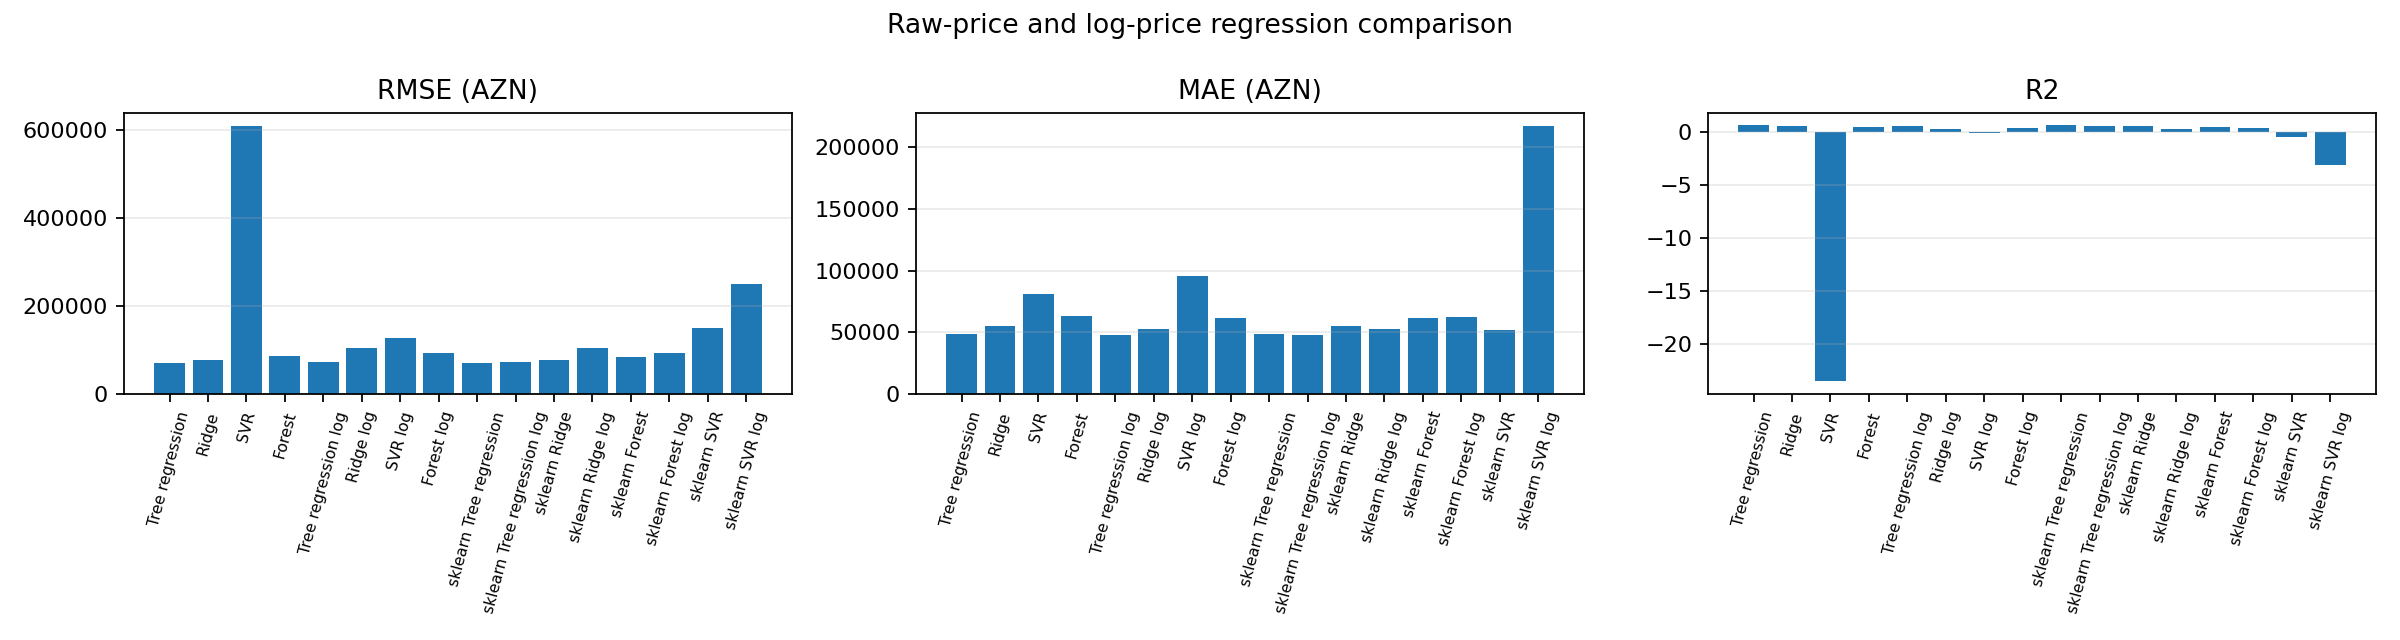
\includegraphics[width=\linewidth]{regression_comparison.png}
  \caption{Comparison of raw and log-price regression models on the test set.}
  \label{fig:regression}
\end{figure}

\noindent
Figure~\ref{fig:classification} summarises the F1 and ROC-AUC values from
Table~\ref{tab:classification}. The custom tree is the strongest custom
classifier.

\begin{figure}[!t]
  \centering
  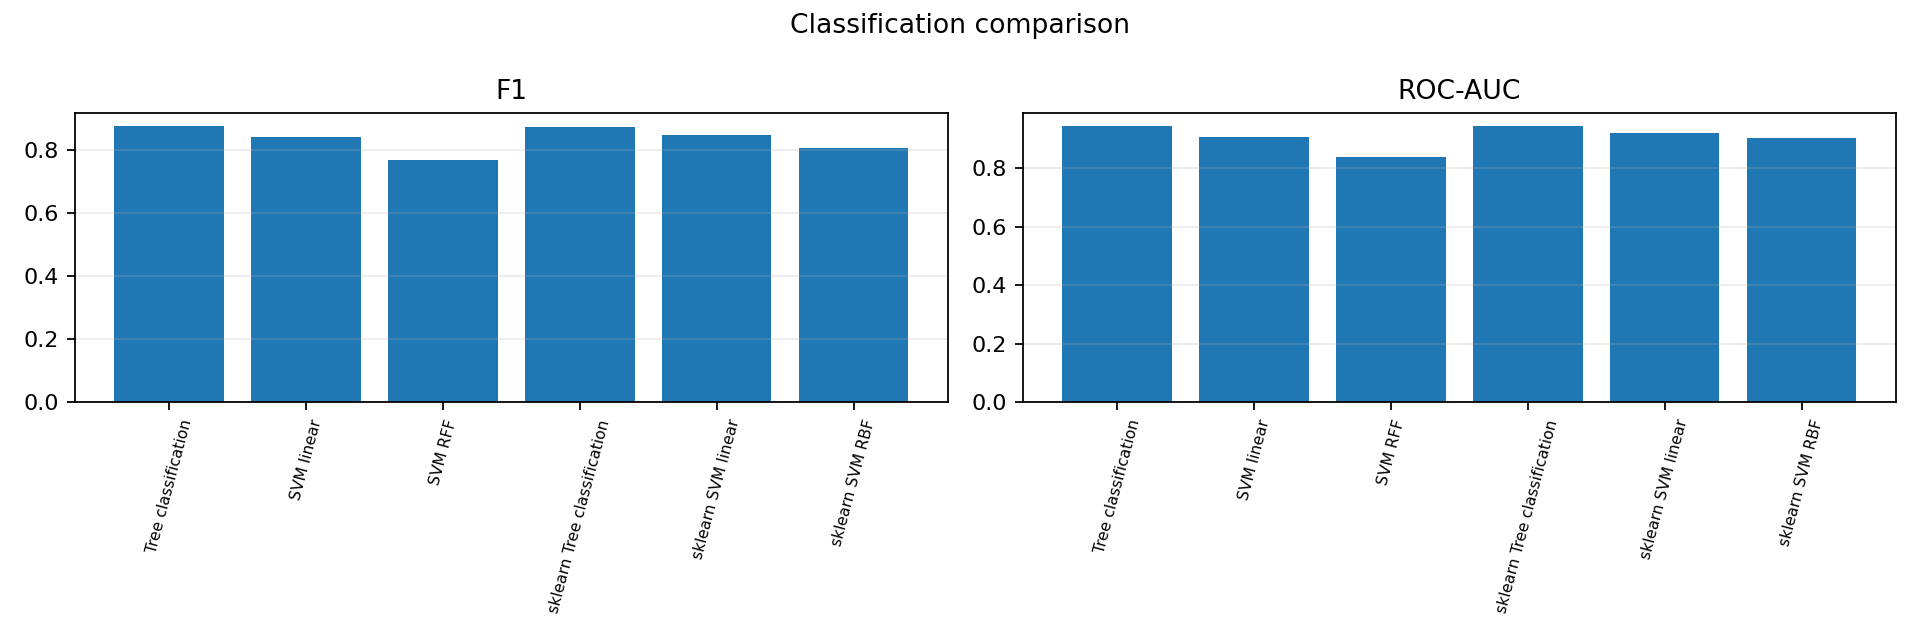
\includegraphics[width=\linewidth]{classification_comparison.png}
  \caption{Classification comparison using F1 and ROC-AUC.}
  \label{fig:classification}
\end{figure}

\begin{figure}[!t]
  \centering
  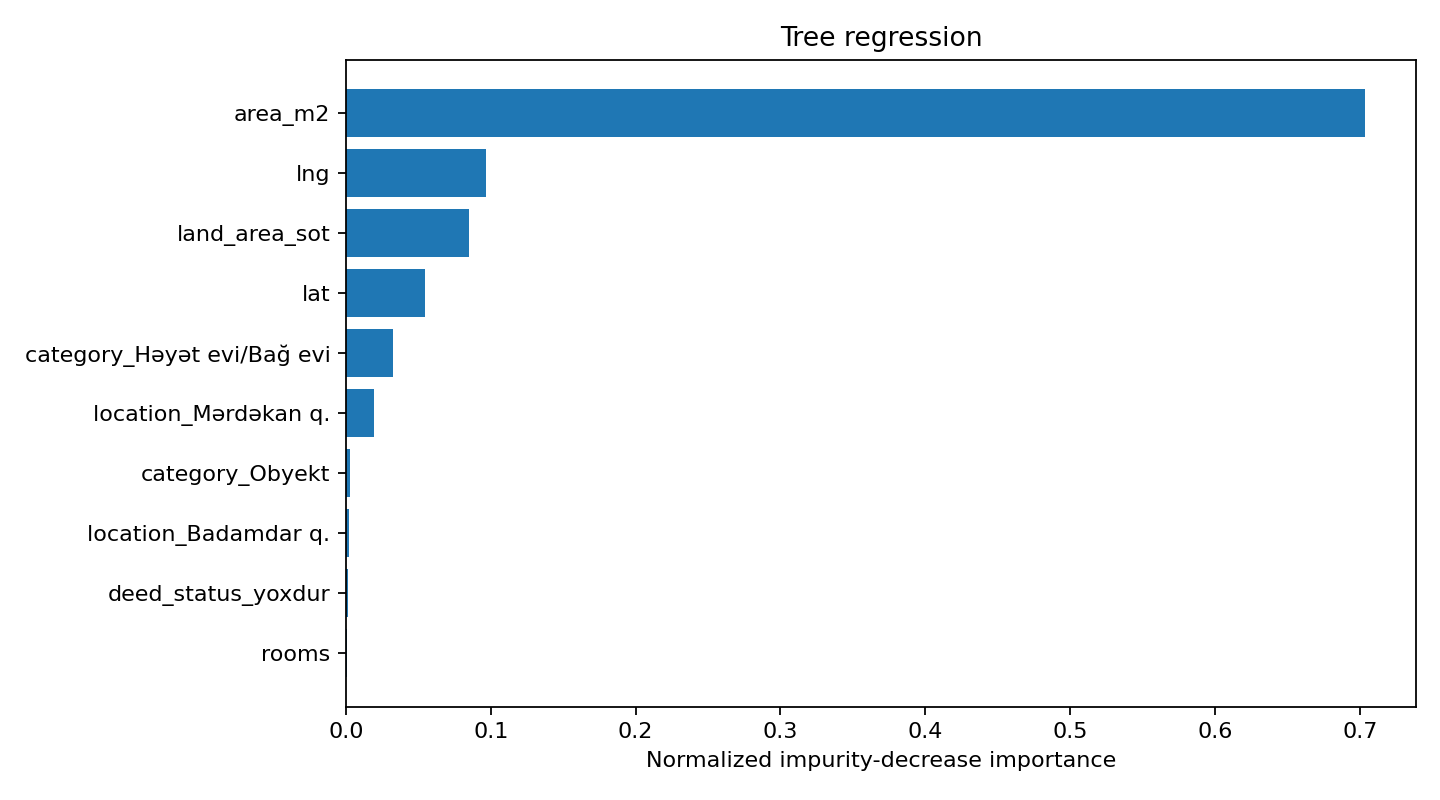
\includegraphics[width=\linewidth]{feature_importance_Tree_regression.png}
  \caption{Feature importance from the selected raw-price tree.}
  \label{fig:importance}
\end{figure}

\begin{figure}[!t]
  \centering
  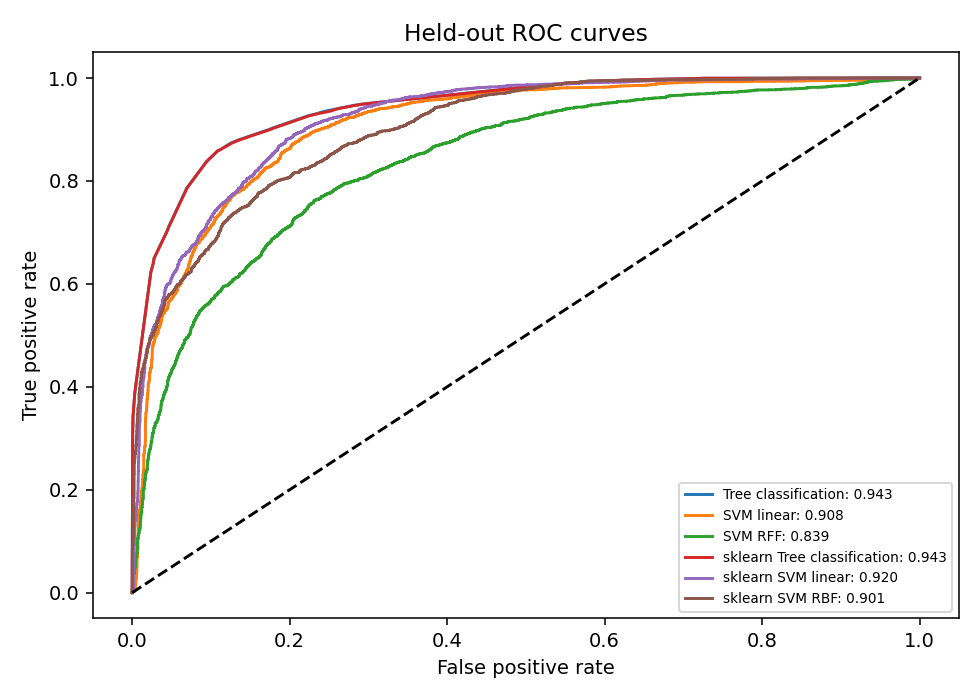
\includegraphics[width=\linewidth]{roc.png}
  \caption{ROC comparison for the classification models.}
  \label{fig:roc}
\end{figure}

Figure~\ref{fig:roc} shows that the tree ranks premium listings well across
thresholds, while the linear and RFF SVMs provide weaker separation.
Figure~\ref{fig:importance} gives a model-specific view of which encoded
listing attributes most influenced the selected tree.
\FloatBarrier

\FloatBarrier

\section{Discussion and Limitations}
The classification task is easier than exact price prediction: the model
only needs to distinguish prices above or below the median. The tree
classifier achieved F1 0.873 and ROC-AUC 0.943, showing strong separation
between the two tiers. The regression tree explained 66.0\% of test-price
variation, but its median absolute error was about 32,651 AZN and its
mean absolute error was about 48,559 AZN.

Errors increased for expensive properties. The tree predicts a leaf mean,
so unusual high-value listings are pulled toward the average of their
leaf and are often underpredicted. The forest was more stable but did not
outperform the selected tree under the tested small configuration. The
SVR variants were weak, while the linear Pegasos SVM was useful for
classification but not used for price regression. The log transformation
did not solve the high-value error problem; it is best viewed here as a
useful comparison rather than the final model.

The difference between regression and classification is also important.
Regression must estimate an exact monetary value, so an error of 100,000
AZN remains large even when the model correctly identifies the broad price
segment. Classification only asks whether the price is above or below
195,000 AZN. This explains why the classification scores are strong while
the price errors remain practically meaningful. In the regression test
set, the median absolute error was approximately 32,651 AZN, but errors
for listings above 500,000 AZN averaged roughly 165,000 AZN. The model
therefore captures broad market structure better than luxury-property
valuation.

The raw and log trees provide a useful robustness comparison. The raw tree
achieved $R^2=0.660$, while the log tree achieved $R^2=0.639$. Their MAE
values were very close (48,559 and 48,313 AZN, respectively). Training on
the logarithm gives relatively more attention to proportional differences,
but inverse transformation does not guarantee lower absolute AZN error.
For this dataset, the raw target is the better headline choice, while the
log model supports the conclusion that the result is not dependent on one
target representation.

The custom tree also almost exactly matches the scikit-learn tree baseline:
their RMSE values are 71,741 and 71,735 AZN, respectively. This agreement
is evidence that the split search and stopping rules are implemented
consistently. It is not evidence that the model is perfect; both models
share the same features, split, and limitations.

These results are conditional on the cleaned dataset and split protocol.
The data contain advertised rather than confirmed transaction prices, and
important details such as exact interior quality and negotiation effects
may be missing. The outlier rule is applied before splitting because the
starter pipeline specifies shared cleaning; this should be stated when
comparing the results with other protocols. Finally, an RMSE of about
71,741 AZN is too large for unsupervised professional valuation, although
the model is suitable for an academic approximate-estimation system.

\section{Conclusion}
The project produced reproducible from-scratch decision tree and Pegasos
SVM implementations and compared them fairly with standard baselines.
The decision tree was the best tested raw-price model, while the tree
classifier was the strongest custom classification model. The results
show that the available listing features contain meaningful price signal,
but exact valuation remains difficult, especially for expensive homes.
Future work should focus on stronger boosting ensembles, safe interaction
features, finer location representations, and evaluation of relative
error and prediction intervals.

\section*{Tools and Acknowledgements}
The team used Python, NumPy, pandas, matplotlib, and scikit-learn for
data processing, plotting, and comparison baselines. The custom decision
tree and Pegasos SVM were implemented without scikit-learn model classes.
Different team members also used Claude, GitHub Copilot (mainly GPT and
Astra-assisted sessions), and Codex for code review, debugging, metric
interpretation, and drafting or editing technical prose. These assistants
were used as support tools rather than as model implementations or sources
of experimental results; the team remains responsible for the code,
experiments, claims, and final report.

\begin{thebibliography}{9}
\bibitem{pegasos}
S.~Shalev-Shwartz, Y.~Singer, Y.~N.~Srebro, and A.~Cotter,
``Pegasos: primal estimated sub-gradient solver for SVM,''
\emph{Mathematical Programming}, vol.~127, no.~1, pp.~3--30, 2011.
\bibitem{cortes1995}
C.~Cortes and V.~Vapnik, ``Support-vector networks,''
\emph{Machine Learning}, vol.~20, pp.~273--297, 1995.
\bibitem{breiman2001}
L.~Breiman, ``Random forests,''
\emph{Machine Learning}, vol.~45, no.~1, pp.~5--32, 2001.
\bibitem{hoerl1970}
A.~E.~Hoerl and R.~W.~Kennard, ``Ridge regression: Biased estimation
for nonorthogonal problems,'' \emph{Technometrics}, vol.~12, no.~1,
pp.~55--67, 1970.
\bibitem{binaaz}
S.~Memmedli, ``Binaaz sale project,'' Kaggle dataset.
\url{https://www.kaggle.com/datasets/sehriyarmemmedli/binaaz-sale-project}.
\bibitem{skdocs}
Scikit-learn developers, ``Scikit-learn User Guide: Support vector
machines, decision trees, ensemble methods, and linear models,''
\url{https://scikit-learn.org/stable/user_guide.html}.
\end{thebibliography}

\end{document}
